\documentclass[runningheads]{llncs}
\usepackage[T1]{fontenc}
\usepackage{graphicx}
\usepackage{booktabs}
\usepackage{url}
\setlength{\emergencystretch}{3em}
\graphicspath{{figures/}}

\makeatletter
\newenvironment{replayfigure}
  {\par\medskip\noindent\begin{minipage}{\linewidth}\centering\def\@captype{figure}}
  {\end{minipage}\par\medskip}
\makeatother

\newcommand{\href}[2]{\leavevmode\pdfstartlink attr{/Border [0 0 0]} user
  {/Subtype /Link /A << /S /URI /URI (#1) >>}#2\pdfendlink}

\begin{document}

\title{Evaluating and Diagnosing Object-Centric Spatial Reasoning in 7B Vision--Language Models}
\titlerunning{Object-Centric Spatial Reasoning in 7B VLMs}
\author{Tran Nguyen-Le\inst{1,2} \and Nhu-Khai Tran\inst{1,2} \and Hong-Anh Dinh-Nguyen\inst{1,2}}
\authorrunning{T. Nguyen-Le et al.}
\institute{Faculty of Information Technology, University of Science, Ho Chi Minh City, Vietnam \and
Vietnam National University, Ho Chi Minh City, Vietnam \\
\email{\{nltran2525, tnkhai2507, dnhanh2511\}@apcs.fitus.edu.vn}}

\maketitle

\begin{abstract}
Real-world 3D spatial reasoning remains challenging for vision--language models even at the 7B scale. This project evaluates five Qwen2.5-VL-based approaches on selected 3DSRBench subtasks: APC-Vis, PCD, SymPL, VST-7B-RL, and Spatial-SSRL-7B. The study contrasts inference-time geometric or decoding interventions with publicly released spatially trained checkpoints. On Left/Right, APC-Vis achieves 81.09\% per-question accuracy, followed by SymPL at 79.08\% and PCD at 76.22\%; their CircularEval scores are 78.22\%, 79.08\%, and 75.07\%, respectively. On Object Facing, APC-Vis and VST reach similar accuracy (71.24\% and 70.95\%) but disagree on many individual examples. Visibility and Front/Behind are evaluated separately. Stored intermediate traces support diagnosis of object selection, orientation, scene transformation, rendering, and final-answer selection. Earlier 3B replay observations are retained as exploratory evidence rather than pooled with the new 7B evaluation.
\end{abstract}

\section{Problem Statement \& Research Questions}

Modern vision--language models perform strongly on conventional 2D visual question answering, but object-centric 3D reasoning requires additional operations: identifying the reference object, determining its facing direction, estimating relative positions, and interpreting relations in a different coordinate frame. The 3DSRBench benchmark provides real-image questions for studying these limitations~\cite{3dsrbench}.

The project now focuses on five methods at the 7B scale, rather than on reducing model size. APC-Vis, PCD, and SymPL intervene at inference time using an unchanged Qwen2.5-VL-7B-Instruct backbone. VST-7B-RL and Spatial-SSRL-7B instead use released checkpoints whose parameters were updated through spatial training. Running these checkpoints on Kaggle allows us to compare external geometric representations and prompting/decoding with spatial knowledge learned during training. We reproduce inference and evaluation, not the training procedures of VST or Spatial-SSRL. A 7B parameter count alone does not establish state-of-the-art performance; conclusions are tied to the evaluated tasks and protocols.

\begin{itemize}
    \item \textbf{RQ1:} How do inference-time methods and spatially trained 7B models compare on the same object-centric spatial questions?
    \item \textbf{RQ2:} Which image characteristics and intermediate decisions explain shared and method-specific errors, including errors hidden by a correct final answer?
    \item \textbf{RQ3:} Which targeted interventions in object selection, orientation, scene representation, or answer selection improve held-out performance without introducing regressions?
\end{itemize}

\section{Reproduction and Evaluation of Five 7B Methods}

\subsection{Experimental Setup}

Experiments use Kaggle runtimes with two NVIDIA T4 GPUs. APC-Vis, PCD, and SymPL use \texttt{Qwen2.5-VL-7B-Instruct}. The trained models are \path{rayruiyang/VST-7B-RL} and \path{internlm/Spatial-SSRL-7B}. The official method name is Spatial-SSRL (Self-Supervised Reinforcement Learning), sometimes abbreviated as Spatial-SRRL in earlier project notes.

The evaluation uses selected 3DSRBench question groups rather than the entire benchmark. Left/Right contains 698 question instances (349 A/B-permutation groups), Front/Behind contains 688 (344 groups), and Object Facing contains 692 (346 groups). Visibility is a separate reformulation of the Front/Behind source questions, also containing 688 instances. APC-Vis and SymPL run Left/Right, Visibility, and Facing; PCD runs Left/Right and Front/Behind; Spatial-SSRL runs Left/Right, Front/Behind, and Facing; VST runs all four protocols. Visibility and Front/Behind are not merged or treated as interchangeable measurements.

The result files contain 10,386 method--question predictions. Matching across models checks the question, answer options, gold answer, image identity, and CircularEval group. Failed executions, invalid answers, and other errors count as wrong. SymPL outputs are normalized to the available options; this recovers 12 Facing answers expressed as object names. The raw responses remain available for auditing. No new direct-Qwen baseline is included in this evaluation, so the results do not estimate a new within-run improvement over an untuned baseline.

\subsection{Method Overview and Data Flow}

\paragraph{APC-Vis~\cite{lee2025perspective}.}
The input image and question are first used to identify relevant objects and the reference viewer. Grounding DINO proposes boxes, Qwen selects the intended instances, SAM produces masks, Depth Pro estimates depth, and Orient Anything estimates orientations. The pipeline constructs a simplified 3D scene, transforms it into the viewer's frame, and renders colored target objects. Qwen answers a reformulated question using the rendered scene, and the answer is mapped back to the original options. The current implementation includes question-subject viewer repair; this was used in 62 evaluated instances. Thus, these are results of the adapted Kaggle pipeline, not an assertion of an unchanged execution of the paper's code.

\paragraph{PCD~\cite{chung-yoon-2026-improving}.}
The image and original viewpoint-dependent question are paired with a camera-view reformulation. A branch-selection prompt determines whether to use the direct camera branch or perspective-conditional contrastive decoding. In the contrastive branch, each option is scored using its log-probability under the original question minus four times its log-probability under the camera-view question. The selected score determines the answer. This involves option scoring as well as prompting; it is not simply two independent text answers. Both branch predictions are retained for diagnosis, and the Front/Behind and Left/Right branch mappings are handled separately.

\paragraph{SymPL~\cite{jang2026sympl}.}
The image and question enter a spatial-information extraction stage: the VLM identifies the reference and target objects, Grounding DINO supplies object regions, Depth Pro supports 3D position estimation, and Orient Anything supplies orientation information. Instead of rendering an egocentric perspective view as APC does, SymPL constructs a symbolic projective layout. For the evaluated tasks, it projects positions into a top-down plane, centers the reference object, and aligns its facing direction upward. Objects become colored symbols. A task-dependent partition separates spatial regions, and the question is rewritten as symbol localization in those regions. Qwen reads the layout and its reformulated question, and the resulting color or object is mapped to an answer option. Its four key operations are projection, abstraction, bipartition, and localization. These transformations require no additional VLM training.

\paragraph{VST-7B-RL~\cite{yang2025vst}.}
Visual Spatial Tuning builds spatial perception through supervised training on VST-P (4.1 million examples spanning 19 skills) and develops reasoning with VST-R (135,000 examples), including a reasoning cold start and reinforcement learning. In our evaluation, training is already encoded in the released checkpoint: the RGB image, question, and options are processed by the Qwen2.5-VL-based model, which generates a reasoning response and final answer. The answer parser extracts the selected option. There is no external detector, depth estimator, orientation model, or scene renderer called by this inference runner. Consequently, its trace consists of model inputs, generated reasoning, final answers, and runtime information, rather than an explicit geometric tool chain.

\paragraph{Spatial-SSRL-7B~\cite{liu2025spatialssrl}.}
Spatial-SSRL trains spatial understanding using verifiable self-supervised tasks derived from RGB or RGB-D images: shuffled patch reordering, flipped patch recognition, cropped patch inpainting, regional depth ordering, and relative 3D position prediction. The paper uses a supervised cold start followed by GRPO, with accuracy and output-format rewards. Our runner loads the released 7B checkpoint and supplies the RGB image, question, options, and reasoning-format instruction. The model emits reasoning inside \texttt{<think>} tags and a final answer in \texttt{\textbackslash boxed\{\}}; the parser maps that answer to the options. The pretext tasks and depth supervision belong to training, not to additional tool calls during benchmark inference. We do not retrain the model on Kaggle.

\subsection{Evaluation Protocol and Results}

Per-question accuracy is the number of correct predictions divided by all evaluated instances. CircularEval counts a group as correct only when both A/B permutations are answered correctly. The two permutations are not independent images. Table~\ref{tab:3dsrbench-summary} reports CircularEval, and Table~\ref{tab:accuracy7b} reports per-question accuracy. All failures count as wrong. Overall scores across different task scopes are not used to rank the methods.

\begin{table}[t]
\centering\small
\setlength{\tabcolsep}{5pt}
\caption{7B CircularEval accuracy (\%) on the evaluated protocols. A dash means the protocol was not evaluated.}
\label{tab:3dsrbench-summary}
\begin{tabular}{@{}lrrrr@{}}
\toprule
Method & Left/Right & Front/Behind & Visibility & Facing \\
\midrule
APC-Vis & 78.22 & -- & 73.84 & 67.63 \\
PCD & 75.07 & 65.99 & -- & -- \\
SymPL & 79.08 & -- & 77.03 & 69.94 \\
VST-7B-RL & 41.55 & 63.08 & 50.00 & 66.18 \\
Spatial-SSRL-7B & 30.95 & 56.98 & -- & 62.43 \\
\bottomrule
\end{tabular}
\end{table}

\begin{table}[t]
\centering\small
\setlength{\tabcolsep}{5pt}
\caption{Per-question accuracy (\%) by task. Fail, invalid, and error count as wrong. A dash means the task was not evaluated.}
\label{tab:accuracy7b}
\begin{tabular}{@{}lrrrr@{}}
\toprule
Model & Left/Right & Front/Behind & Visibility & Facing \\
\midrule
APC-Vis & 81.09 & -- & 74.71 & 71.24 \\
PCD & 76.22 & 69.77 & -- & -- \\
SymPL & 79.08 & -- & 77.03 & 69.94 \\
VST-7B-RL & 46.13 & 66.42 & 52.33 & 70.95 \\
Spatial-SSRL-7B & 33.81 & 62.06 & -- & 69.22 \\
\bottomrule
\end{tabular}
\end{table}

APC-Vis has the highest per-question Left/Right accuracy in these runs, whereas SymPL has the highest CircularEval score. SymPL also leads Visibility. On the original Front/Behind protocol, PCD outperforms VST and Spatial-SSRL. Facing is substantially closer across methods: APC-Vis and VST differ by only two correct instances (493 versus 491), but APC alone is correct on 133 instances and VST alone on 131. Their similar aggregate scores therefore conceal different failure sets.

The new APC diagnostic replay contains 120 selected instances: 40 per task, comprising 28 wrong and 12 correct answers. Replay predictions agree with the corresponding benchmark predictions. This intentionally selected set supports qualitative analysis but is not used to estimate error prevalence. The older 3B replay examples in Section~3 are kept separate from these 7B results.

\raggedbottom
\section{Observations and Hypotheses}

\subsection{Observations}

\par\medskip\noindent\begin{minipage}{\linewidth}
\paragraph{1. Incorrect object localization can produce an unreliable scene.}
APC-Vis builds its scene from detected object regions. If a region points to the wrong object, the estimated position and orientation describe that region rather than the intended object. In Q793LOEX, the question asks whether the kitchen paper towel is on the woman's left or right. The selected paper-towel region lies over the microwave area. However, the current 7B run answers correctly. This is an intermediate localization error hidden by a correct final answer, not a confirmed wrong-answer example. A returned box should therefore be checked for object identity, not just for its existence.

\begin{replayfigure}
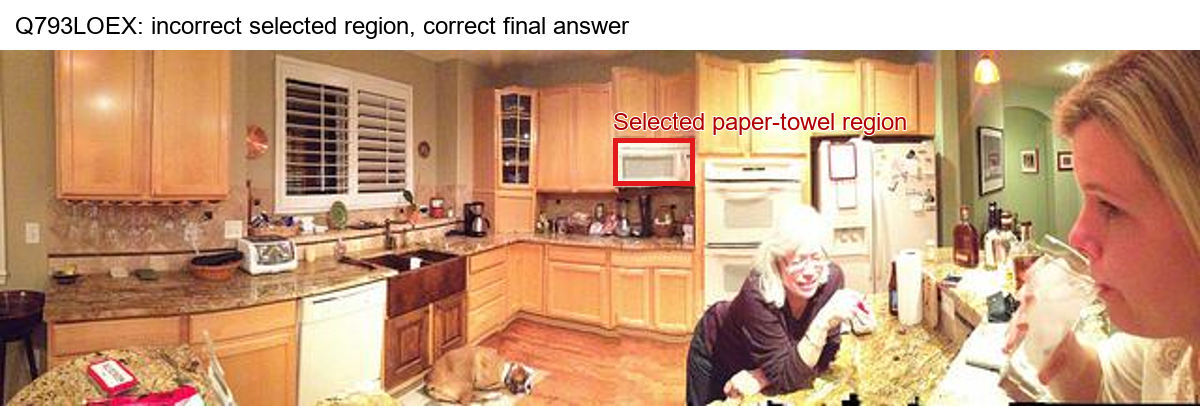
\includegraphics[width=\linewidth]{observation-paper-towel.png}
\caption{Q793LOEX (7B, instance 5486). Red marks the region used for the kitchen paper towel; it overlaps the microwave area. The final answer is correct despite this incorrect region.}
\end{replayfigure}
\end{minipage}\par


\par\medskip\noindent\begin{minipage}{\linewidth}
\paragraph{2. Objects cut off by the image boundary are difficult to locate.}
In 6VD7EBFE, the question asks whether the picture on the wall faces the fridge or the microwave. APC-Vis selects the microwave, while the annotated answer is the fridge. Only a narrow part of the fridge is visible at the right boundary. This makes object localization a plausible source of error. The original-image detection trace is unavailable, so we cannot yet distinguish a missed detection from an incorrect box, orientation, or scene estimate. The horizontally flipped version is answered correctly, indicating sensitivity to the image transformation.

\begin{replayfigure}
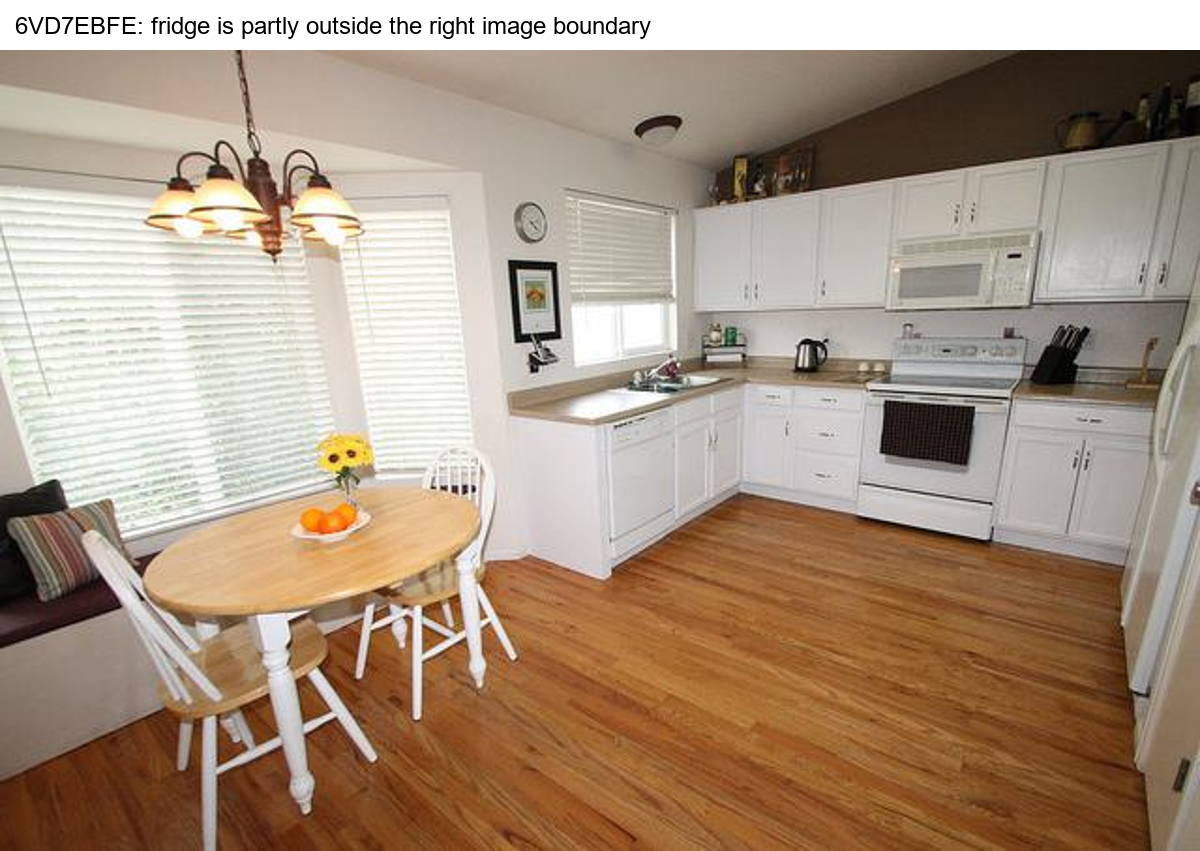
\includegraphics[width=.82\linewidth]{observation-fridge.png}
\caption{6VD7EBFE (7B, instances 8296--8297). The fridge is partly outside the image. Gold answer: fridge; APC-Vis answer: microwave. Detection failure is suspected, not established from the available trace.}
\end{replayfigure}
\end{minipage}\par


\par\medskip\noindent\begin{minipage}{\linewidth}
\paragraph{3. Orientation estimates can be unstable.}
A correct object region does not guarantee a correct facing direction. In an earlier 3B-pipeline replay, Orient Anything's predictions for a dog and its horizontally flipped image differ by approximately 167 degrees after accounting for the reflection. This demonstrates inconsistency, although it does not identify which prediction is correct. If an inconsistent orientation is used for the reference viewer, the transformed scene can also become incorrect.

\begin{replayfigure}
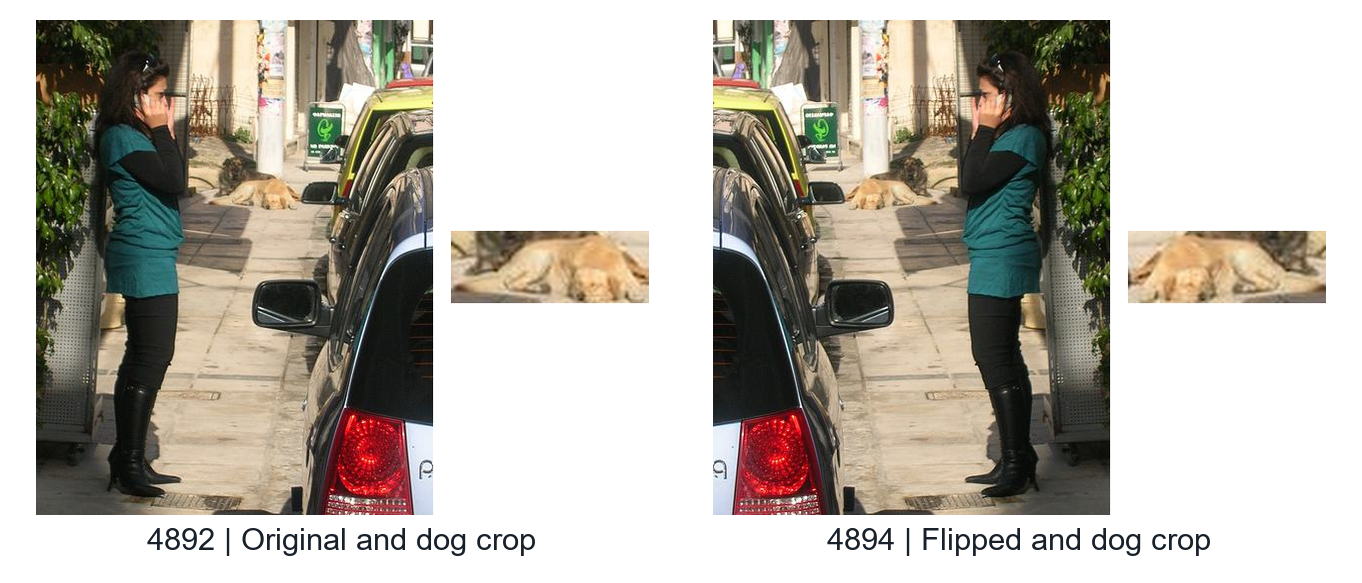
\includegraphics[width=\linewidth,height=45mm,keepaspectratio]{failure-orientation-flip.png}
\caption{Earlier replay instances 4892 and 4894: the dog orientation is inconsistent under horizontal reflection. This is an orientation-consistency example from the previous diagnostic study, not an error-rate estimate for the new 7B runs.}
\end{replayfigure}
\end{minipage}\par


\par\medskip\noindent\begin{minipage}{\linewidth}
\paragraph{4. PCD may select the wrong branch.}
In the current 7B evaluation, PCD gives 374 wrong answers. For 357 of these instances, the alternative branch gives the correct answer. The remaining 17 are wrong in both branches. This suggests that branch selection is a useful improvement target, but selecting a branch using the gold answer would not be a valid inference method.

\begin{replayfigure}
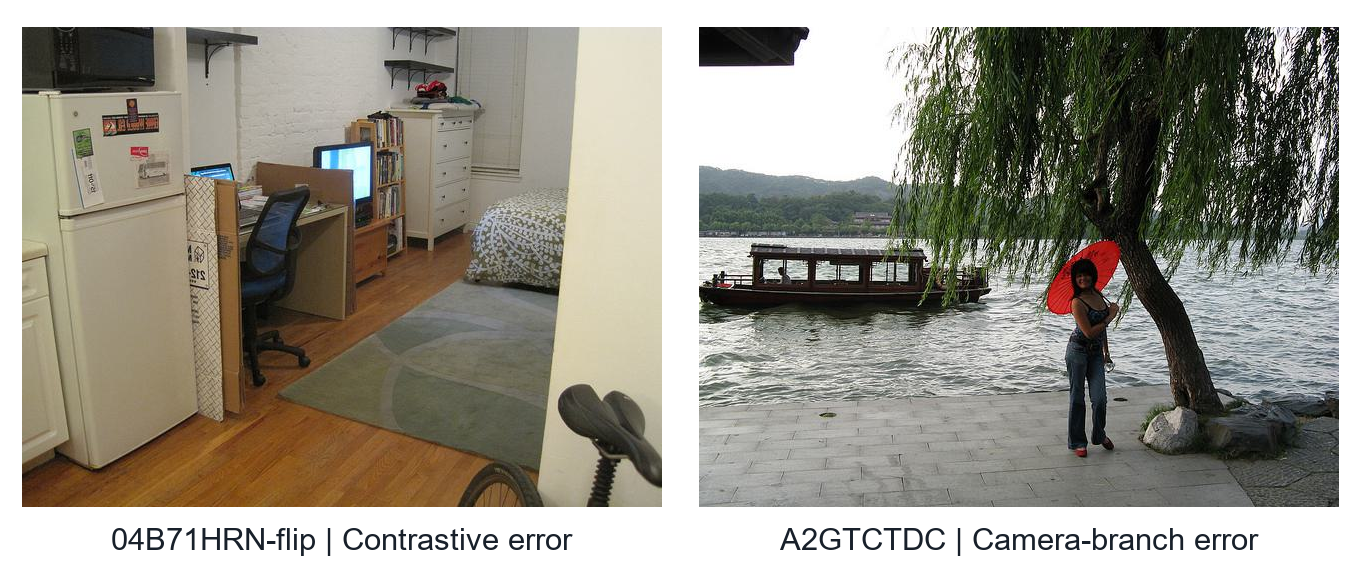
\includegraphics[width=\linewidth,height=43mm,keepaspectratio]{failure-pcd-branches.png}
\caption{Examples from the earlier PCD replay illustrate the two possible routing errors: selecting the contrastive branch when the camera branch is correct, and vice versa. The 357/374 count above comes from the new 7B evaluation, not from these illustrative examples.}
\end{replayfigure}
\end{minipage}\par


\subsection{Hypotheses and Simple Validation Plan}

\paragraph{H1. Joint 3D reconstruction and object detection may improve APC-Vis.}
Our working hypothesis is that incorrect object localization and Orient Anything estimates are major sources of APC-Vis errors. The examples motivate this hypothesis, but do not establish that these components explain most failures. Instead of separately detecting 2D boxes, estimating depth, and predicting orientation from crops, a model could reconstruct the scene and predict oriented 3D bounding boxes within a shared coordinate system. More consistent object positions and orientations may produce better viewpoint transformations and answers.

To test this idea, compare the existing pipeline with a reconstructed-scene pipeline on the same held-out questions, keeping the final VLM and answer protocol fixed. First replace only object localization, then orientation, and finally both. Report object recall, box quality, orientation consistency, and final accuracy, including answers that change from correct to wrong. Include cropped, occluded, and small objects as separate groups. A 3D box axis is not automatically the object's semantic facing direction; the new model must also identify the front of the object. Reconstructing a single image may still fail when an object is barely visible or outside the frame.

\paragraph{H2. A better branch selector may improve PCD.}
Compare the current selector with always using the camera branch and always using the contrastive branch. Develop a new selector using only information available at inference, then evaluate it on held-out question groups. Keep A/B permutations and flipped versions of the same example in the same split.

\section{Plan for Next Week}

The next stage will focus on the following activities:

\begin{enumerate}
    \item \textbf{Compare accuracy at the subtask level.} Extend the five-method comparison in Section~2 with controlled, subtask-specific ablations. Report per-subtask accuracy and CircularEval, while clearly distinguishing APC Visibility from PCD Front/Behind.
    \item \textbf{Analyze the trained checkpoints.} Use the completed VST-7B-RL and Spatial-SSRL-7B evaluations to compare shared and method-specific failure cases. Audit prompting and answer parsing before attributing differences to training; no local retraining is planned in this step.
    \item \textbf{Validate the proposed hypotheses.} Begin controlled experiments for H1--H2, using development data to fix rules and held-out groups for evaluation. Report both improvements and regressions, including incorrect-to-correct and correct-to-incorrect transitions.
\end{enumerate}

\bibliographystyle{splncs04}
\bibliography{references}

\end{document}
